\newpage
\section{実験方法}
\subsection{実験環境}
実験環境として\figref{fig:topo}に示す千葉工業大学 2 号館 3 階を用いる.
環境中には,三叉路が 6 つ,角が 3 つ,突き当りが 4 つ含まれている.
また,経路追従モジュールと通路分類モジュールの学習データを収集するために,\figref{fig:route}に示すルートを走行する.

\begin{figure}[htbp]
  \centering
  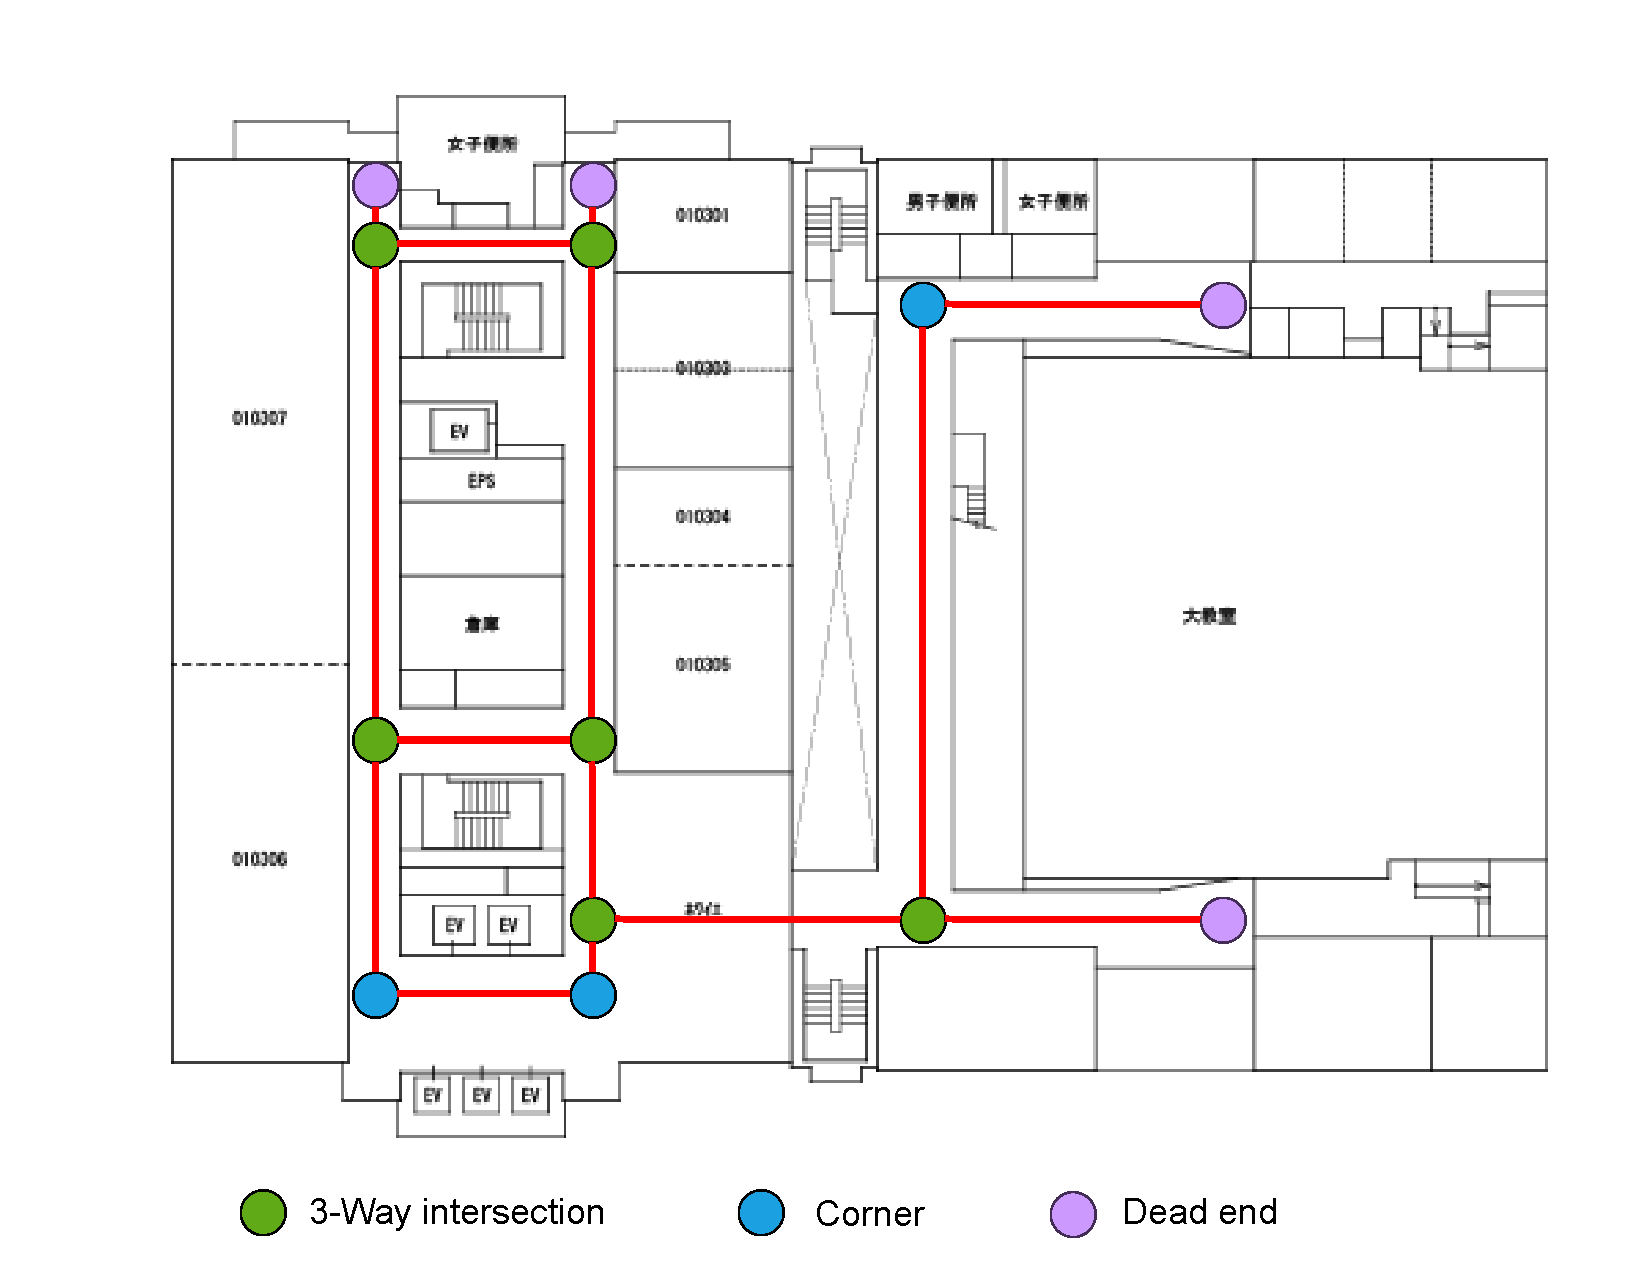
\includegraphics[width=130mm]{images/pdf/ishiguro/topo.pdf}
  \caption{Experimental environment}
  \label{fig:topo}
\end{figure}

\begin{figure}[h]
  \centering
  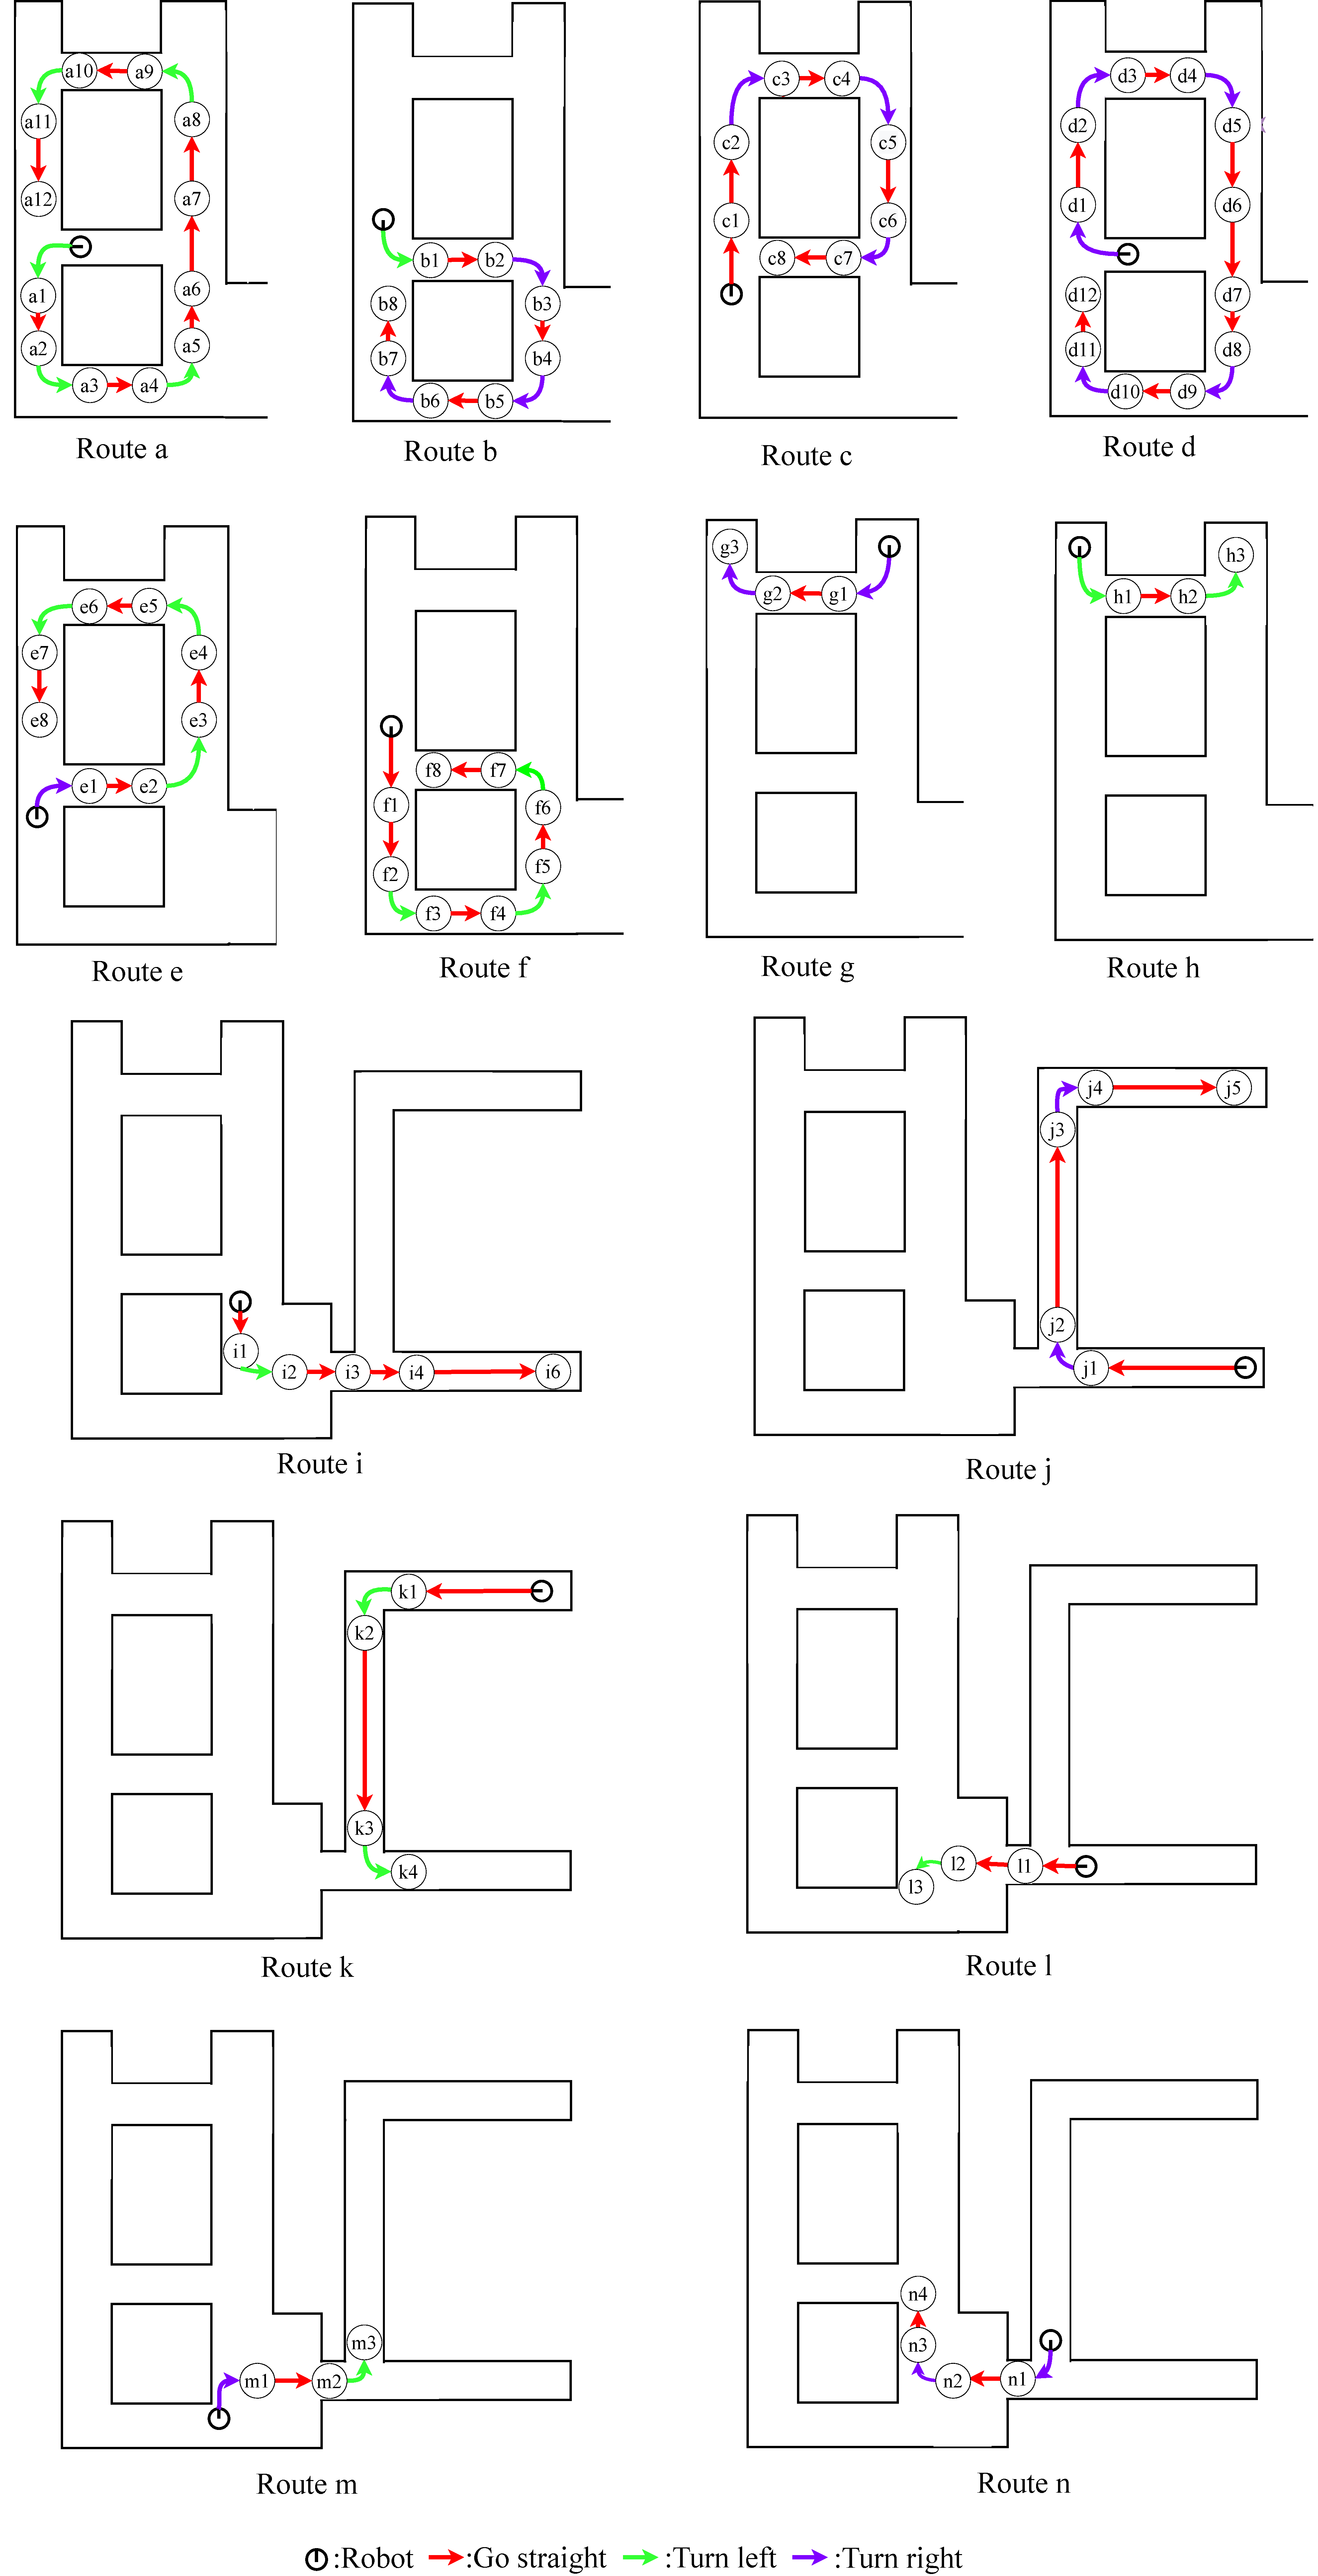
\includegraphics[width=100mm]{images/pdf/ishiguro/route.pdf}
  \caption{Route used for learning}
  \label{fig:route}
\end{figure}

\newpage
\subsection{シナリオの選定}
実験に使用するシナリオを,島田らが作成した 50 例から選定した.
選定するにあたって,以下の条件を設定した.

\begin{enumerate}
  \item [1)] ロボットが移動するには通路が狭すぎて,衝突せずに走行するのが困難な,\figref{fig:keepout}上部に示す部分を走行ルートに含まれないこと.
  \item [2)] 現時点の経路追従モジュールでは対応していない,「後ろを向く」などその場での旋回が含まれていないこと.
  \item [3)] ロボットが移動しても,カメラ画像の特徴の変化が小さいため,通路の種類の分類が困難な\figref{fig:keepout}下部に示す部分がスタート地点では無いこと.
  \item [3)] スタート地点が\figref{fig:keepout}に示す箇所でないこと.この箇所がスタート地点のシナリオは,「左手に通路が見えるまで直進」「右手に通路が見えるまで直進」である.現時点の路分類モジュールの入力である正面のカメラ画像からでは,ロボットが移動してもカメラ画像の特徴の変化が小さく,シナリオの条件を満たす通路分類結果が得られない可能性がある.
\end{enumerate}

条件ごとの除外したシナリオ数を\tabref{tab:remove}に示す.
また,条件 2 と 3 の両方を満たしたシナリオが 2 つある. 
これにより,選定されたシナリオ数は 28 例となる.
\begin{table}[htbp]
  \centering
  \caption{Number of scenarios excluded}\label{tab:remove}
  \begin{tabular}{c|c}
  \hline
  reason & number of secnario\\
  \hline
  1  & 4\\
  2  & 7\\
  3  & 13\\
  \hline
  \end{tabular}
\end{table}

\begin{figure}
  \centering
  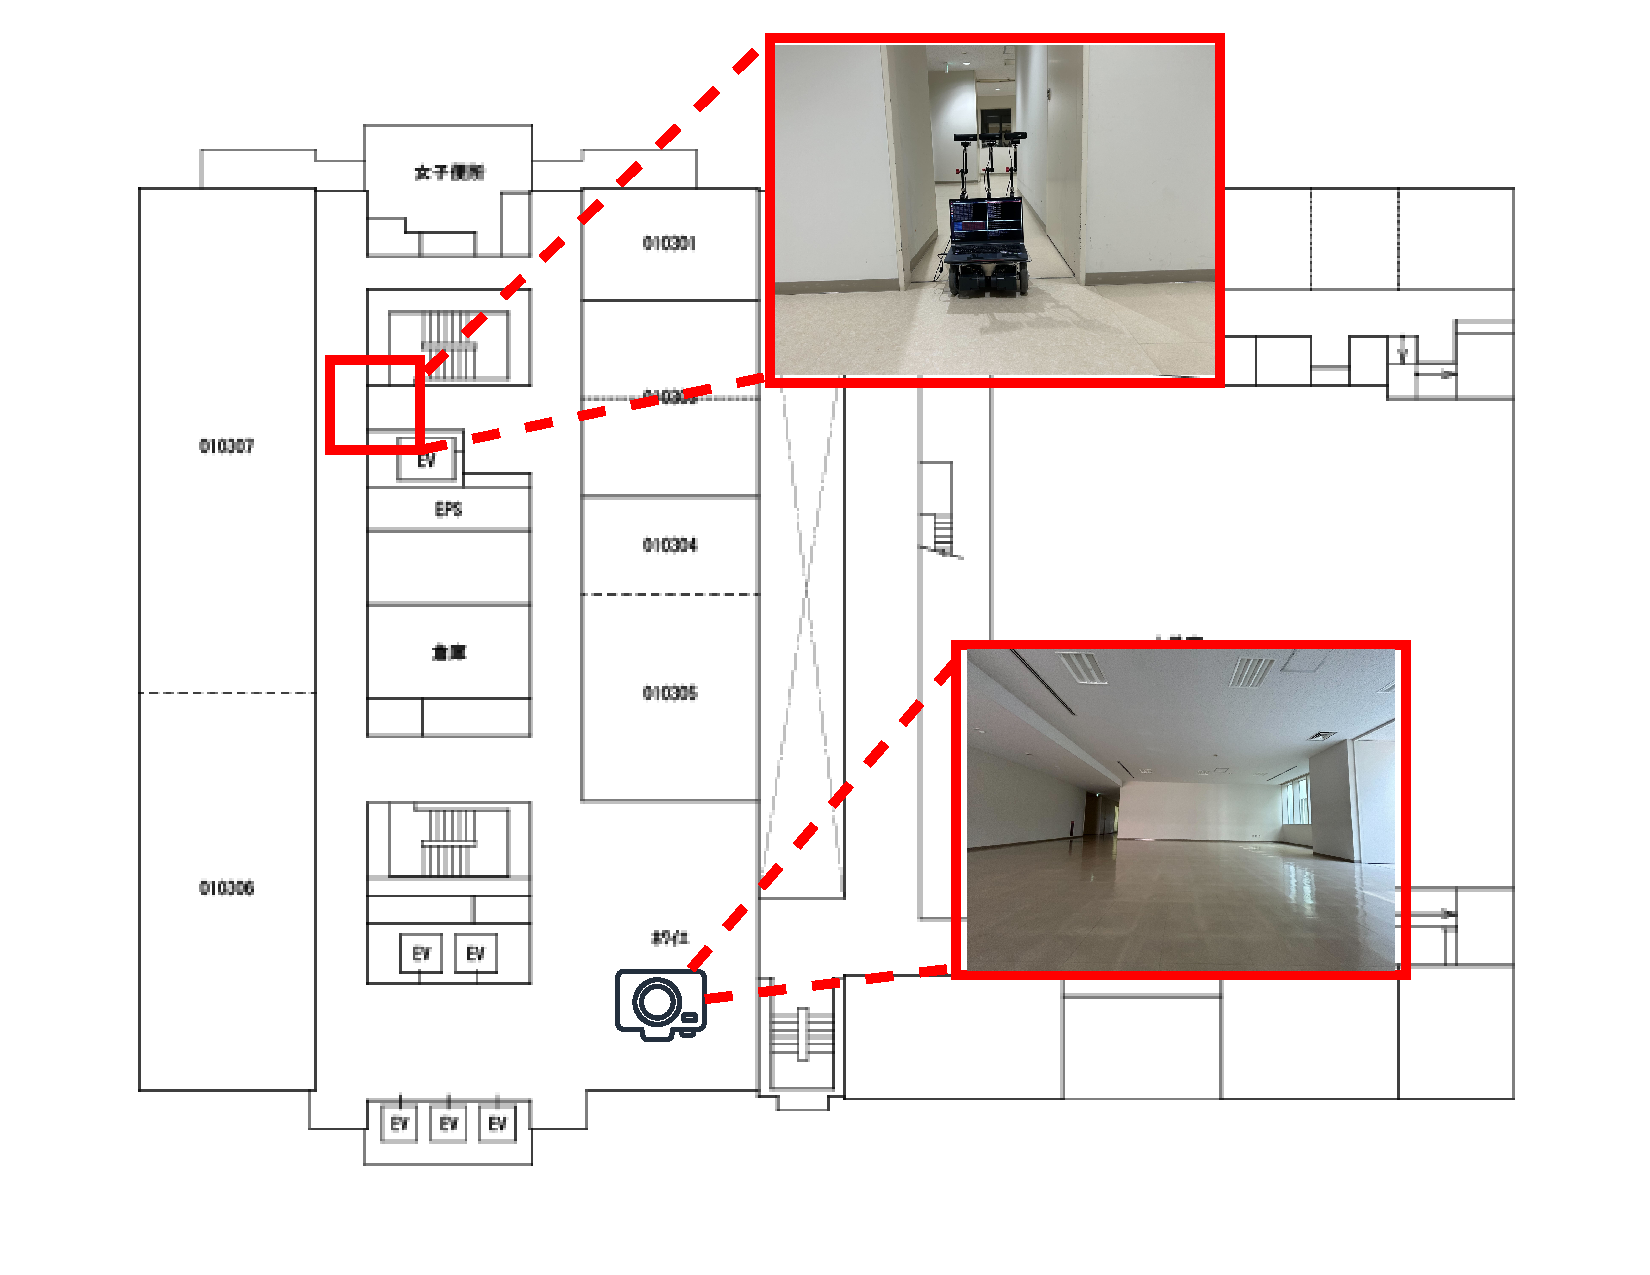
\includegraphics[width=130mm]{images/pdf/ishiguro/keepout.pdf}
  \caption{Experimenta}
  \label{fig:keepout}
\end{figure}

\clearpage
\subsection{経路追従モジュールの訓練}
\figref{fig:route}に示すルートをオンライン学習させながら 1 周走行する.
データセットの収集には藤原ら\cite{fujiwara2023}が提案する手法を用いる.
また,オンライン学習で作成したモデルに追加でオフライン学習を行う.
オフライン学習時のデータセットにはオンライン学習の際に作成したルート 1 周分のデータを用いる.
データセットからはオンライン学習と同様のバッチサイズ 8 でデータをランダムに取得し,epoch数は 20 とした.

\subsection{通路分類モジュールの訓練}
\figref{fig:route}に示すルートをROS の navigation パッケージを使用して,経路を 1 周する.
その際, 3 つのカメラからそれぞれ画像データを収集しながら走行する.
学習時のパラメータとして,バッチサイズを 32 ,epoch数を 30 とし,コストアプローチに用いた重みは\tabref{tab:cost}に示す.

\begin{table}[htbp]
  \centering
  \caption{The weights assigned to each class in the experiment}\label{tab:cost}
  \begin{tabular}{c|c}
  \hline
  Class & Class weights\\
  \hline
  直進   & 1\\
  突き当たり   & 39.5\\
  角(右) & 14\\
  角(左)& 14.2 \\
  十字路 & 1  \\
  三叉路(右)& 6.6  \\
  三叉路(中央)& 7.0  \\
  三叉路(左) & 6.4  \\
  \hline
  \end{tabular}
\end{table}

\clearpage
\subsection{シナリオに基づくナビゲーション}
2 つのモジュールを訓練後,ロボットが目的地まで到達できるか確認する.
実験では,ロボットをシナリオのスタート地点,向きに配置し,シナリオを 1 例ずつ入力する.
壁に衝突することなく正しい経路を選択し,目的地で停止した場合に成功とする.